\documentclass[submit,techrep,noauthor]{ipsj}

\usepackage[dvipdfmx]{graphicx}
\usepackage{latexsym}
\usepackage{url}
\usepackage{xcolor}
\usepackage{listings}
\usepackage{amsmath,amssymb}

\newcommand{\todo}[1]{\colorbox{yellow}{{\bf TODO}:}{\color{red} {\textbf{[#1]}}}}
\newcommand{\memo}[1]{\colorbox{pink}{{\bf MEMO}:}{\color{black} {\textbf{[#1]}}}}
\newcommand{\ihara}[1]{\colorbox{green}{{\bf IHARA}:}{\color{blue} {\textbf{[#1]}}}}

\def\Underline{\setbox0\hbox\bgroup\let\\\endUnderline}
\def\endUnderline{\vphantom{y}\egroup\smash{\underline{\box0}}\\}
\def\|{\verb|}
%

%\setcounter{巻数}{59}%vol59=2018
%\setcounter{号数}{10}
%\setcounter{page}{1}


\begin{document}


\title{大規模言語モデルによるコード生成のための反復的な要件統合と最適化プロセス\\}

\affiliate{IPSJ}{情報処理学会\\
IPSJ, Chiyoda, Tokyo 101--0062, Japan}


\paffiliate{JU}{情報処理大学\\
Johoshori Uniersity}

\author{豊嶋 浩基}{Toyoshima Hiroki}{WU}[s276157@wakayama-u.ac.jp]
\author{伊原 彰紀}{Ihara Akinori}{WU}[ihara@wakayama-u.ac.jp]
\author{田井 聖凪}{Tai Sena}{WU}[s2310137@wakayama-u.ac.jp]

\begin{abstract}
大規模言語モデル (LLM) はソフトウェア開発自動化に大きく貢献するが,複雑な要件を持つソフトウェア開発の実現には課題が多い.本研究は,自然言語からソースコードを自動生成するマルチエージェント型フレームワークChatDevを用いて,few-shotを用いた要件の細分化と要件の統合による反復的に進める開発プロセスを提案する.ケーススタディとして,\todo{競技プログラミングコンテストAtCoderの問題を題材に...結果,XXを明らかにした.}
% と段階的開発を実施した.これにより,入出力テストに基づいた性能の向上が確認できた一方で,局所的な最適化に留まり,システム全体の品質に課題を残す.
% そのため本研究では,分割された要件の統合と反復的改善の概念を組み合わせた新たな開発プロセスを提案する.具体的には,分割・生成されたコード群を対象に,全体の整合性を評価し,再統合と洗練を行うイテレーションを導入する.この反復的な最適化プロセスは,複雑なソフトウェア要件に対するコード生成品質を一段階引き上げるための,新たな開発指針となることを目指す.
\end{abstract}

\maketitle

%%%%%%%%%%%%%%%%%%%%%%%%%%%
%1
\section{はじめに}
%%%%%%%%%%%%%%%%%%%%%%%%%%%

大規模言語モデル (LLM) 技術の急速な発展に伴い\cite{Growing_LLM},LLMはこれまで人間が時間や労力をかけていたタスクの自動化を実現し,幅広い分野の作業を効率化する技術として関心を集めている.ソフトウェア開発においても,コードレビュー,リファクタリング,テストケース生成など,様々な場面において飛躍的に生産性を向上することが確認されている.\cite{LLM_CodeReview}\cite{LLM_Refactoring}\cite{LLM_Gene_Test}その中でも,開発者の意図や要件をプロンプトとして提示し,ソースコードの自動生成には期待が大きい.\cite{LLM_CodeGeneration}

LLMは,自然言語で記述された要求文に基づきソースコードの自動生成を実現し,昨今では複雑で,大規模なソフトウェア開発の自動化に向けた研究が進められている.\cite{LLM_CodeGeneration} 一部の要求は実現できる一方で,複数のソフトウェア要件が内包し,それぞれが相互に依存し合う大規模なソフトウェア要件を満たすソースコード生成には課題が多い\todo{引用}.従来研究ではソフトウェア要件が複雑になると,LLMが十分に推論せずに,短絡的なソースコードを生成する.例えば,仕様の一部が欠損している場合や,要件の文脈を正しく理解できていない場合には,ロジック誤りが生じることがある.これは,要件文から要求を抽出し,それらを基にコードを生成する,という流れをLLMが実施するが,複雑な要件からコードを生成する場合,LLMは追加の情報無しに正しく要求を抽出する事が困難であることが原因の1つであると考えられる.

LLMの理解や推論を補助するプロンプト技術として,思考の過程を明示的に示すChain of Thought (CoT) や,要求を満たす例を少数提示するfew-shot学習が用いられているが,\cite{LLM_fewshot} これらは局所的な推論の補完や思考パターンの学習には有効である一方で,プログラミング言語のように記述方法や実装方法によって同一の要件に対して多様な解が存在する領域では,これらの手法のみでは十分な性能を発揮しにくい.

これに対して先行研究では,全体の流れをfew-shot学習を用いて要件を抽出するフェーズと,それらを基にコードを生成するフェーズの2つに分割する手法が取り入れられており.\cite{tosem} 前者では,大量のデータ収集やそれに対するラベリング,再学習などを要するファインチューニングと比較して,追加学習をようさずにLLM挙動を制御できることからfew-shot学習が採用されている.

\todo{断片化してしまう事を書き漏れてる.TOSEMでは断片化するから,できる限り一括でやるone-shot構造が望ましいって話があったはず.}

\memo{また,関数呼び出しやデータ型・構造などのインタフェースの不一致により,システム全体の整合性が破綻することもある.\todo{全体整合ってなんだろう?}}

以上のことから,本研究では要求抽出の不安定さや,段階的開発におけるコードの断片化対して,複雑な要件の細分化および,細分化した要件ごとの開発における全体整合を実施することでソースコード自動生成を実現する.さらに,細分化した要件をベースとして生成したソースコードを評価し,要件の統合と再分割によるソースコード自動生成を複数回繰り返すことでプロンプト作成の最適化を目指す開発プロセスを提案する.本手法により,各工程下でLLMに対して全体概要を明示的に提示や,分割した要件の統合と再分割を繰り返すことで,マルチエージェント型コード自動生成の品質を向上を期待する.

\todo{場合によっては,ここでRQを紹介する可能性あり}

論文構成は以下の通りである.\ref{sec:related}章で本研究で使用するフレームワークやキーアイディアのベースとなる関連研究について,\ref{sec:method}章ではそれらに基づいたアプローチを述べ,\ref{sec:evaluation}章でそのアプローチに関する実験設定やRQを列挙し,\ref{sec:result}章でそれに対する結果を提示する.\ref{sec:discussion}章で考察と妥当性の脅威について議論した上で,\ref{sec:conclusion}章で結論を述べる.


%%%%%%%%%%%%%%%%%%%%%%%%%%%
%2
\section{関連研究}
\label{sec:related}
%%%%%%%%%%%%%%%%%%%%%%%%%%%

%2.1
\subsection{ChatDev: マルチエージェントによる段階的開発フレームワーク}
LLMを活用したソフトウェア開発を自動化を目的としたシステムとして,MetaGPT,AutoDevなどの開発が盛んに進められている\cite{metagpt} \cite{autodev}.本システムは,ソフトウェア開発プロセスにおける各工程(要求定義,設計,実装,テスト,保守)を自然言語理解と生成能力により自動化する仕組みである.本研究では,各工程の役割を担うLLMエージェントがそれぞれ要件定義から実装までを実現するChatDev\cite{qian-etal-2024-chatdev}を用いる.

ChatDevは,要件定義,設計,実装をウォーターフォールモデルに則って開発を進める過程で,各工程においてプログラマやプロダクトマネージャといった役割を与えられた2つのLLMエージェントが対話しながら開発を行うプラットフォームである.各工程では,開発を担当するエージェントが,プロンプトで与えられた要件文,または前工程で生成された成果物(ソースコードやそこに含まれるコメントなど)に基づき,新たな成果物を生成する.生成した成果物は別の検証を担当するエージェントと共有される.共有を受けたエージェントは,成果物を検証し,開発と検証を担当するエージェント間で合意形成を図って,成果物を完成する.

ChatDevの枠組みは,各工程のタスクが明確である点や,フレームワークがオープンソースとして公開されており,自体の構造の確認,書き換えが可能であるため,拡張性に優れている.一方で,各工程で開発を担当するLLMに対して,同一の要件(プロンプト)が与えられるため,多数の機能を内包するような複雑・大規模な要件の場合,各フェーズでのタスクの粒度が大きくなり,不完全なコードが生成されやすくなってしまう.


%2.2
\subsection{LLMによるソフトウェア開発自動化の課題}
Shojaeeら\cite{IllusionApple}は,複雑度の制御が可能かつ,解法が明確な数学的パズル問題を用いて,LLMの最終的な解とそこに至るまでの推論過程を調査した.その結果,難易度が上昇するにつれて正答率は緩やかに低下すると同時に,複雑度が一定の閾値を超えるまでは推論過程でのテキスト長が増加するのに対して,閾値を超えた場合には急激に低下し,LLMの推論精度が低下する.加えて,推論過程の調査により,複雑度が低い場合に正解には早く到達するが,その後も不要に探索を続けてしまう過剰な推論ステップを踏んでしまう事が確認されており,このようなLLMの挙動は,高い推論能力を要する自然言語からのコード自動生成においても同様に再現されうるものである.複数の要求を内包する複雑な要件文からは,依存関係の見落としや,断片化したコードの生成により,全体整合性の破綻が発生しやすい.

Jiangら\cite{tosem}は,few-shotによりLLMを用いて要件文から小さな実装単位の小要件へ分割を行う「計画フェーズ」と,分割後の要件を基に開発を行なっていく実装フェーズを組み合わせた手法を提案している.

計画フェーズにおいて分割例をfew-shotで提示する事で分割の粒度の統一を目指し,実装フェーズにおいて分割した小要件から各々で断片的に開発を実施するのではなく,分割した要件を実装のガイドとして扱い,コード生成は一度に生成する構造がもっとも高性能であると報告している.これは,要件からコード断片を複数生成し,最終的に結合を行う方式は,コンテキストの欠如により,インタフェースやデータ構造の不整合が発生しやすいことが主な原因であると言及している.

以上を踏まえ,本研究は分割後要件の最適化を図る「要件の細分化」と「細分化後要件の統合と再分割」は,LLMの推論の最適化プロセスの1つとして重要である.
\todo{実装フェーズはただ報告しただけ感が強い.「こうは言ってるけど,ChatDevみたいな構造なら断片化させずに開発できるんじゃ?」みたいな方針を示すように書きたい.}

\ihara{ここまで確認済み}

%%%%%%%%%%%%%%%%%%%%%%%%%%%
%3
\section{要件分割と要件統合に基づく段階的ソースコード生成}
\label{sec:method}
%%%%%%%%%%%%%%%%%%%%%%%%%%%

%--------------------
\begin{figure*}[t]
    \centering
    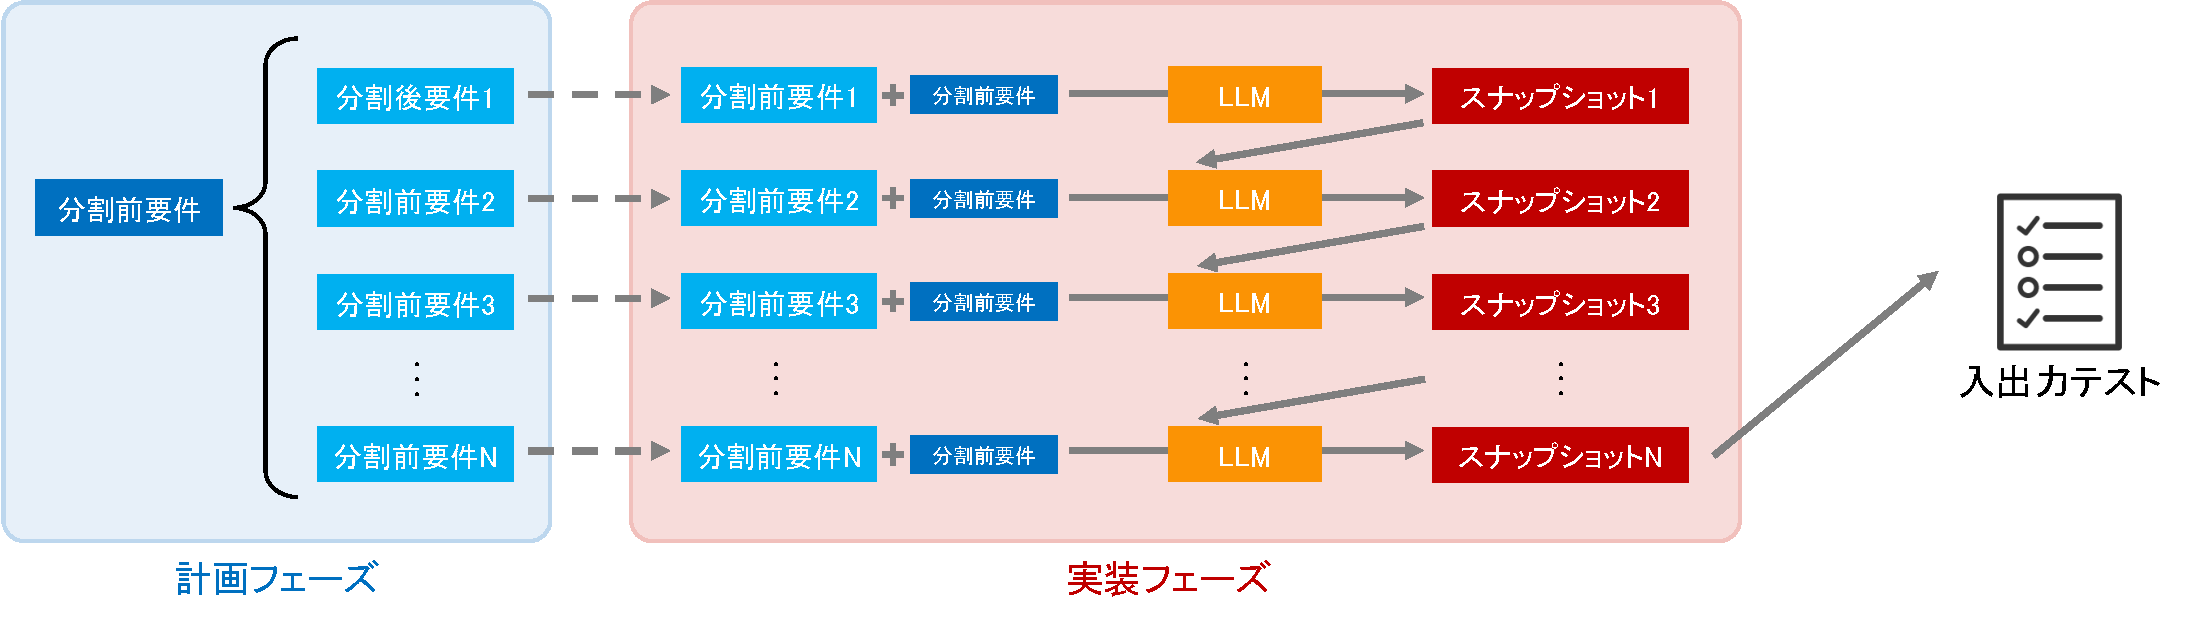
\includegraphics[width=1.0\linewidth]{./Toyoshima_fig/approach_abst_v2.pdf}
    \caption{few-shotと全体概要の有無におけるテスト通過率比較\todo{図タイトル変更}
    \todo{分割前は「要求文」,分割後を「要件文」と区別してはどうでしょう?}\todo{要件からLLMには矢印ではなく通り過ぎるだけ?}\todo{この図には,統合やイテレーションの様子は掲載しないの?}\todo{図中に$S_i$も書く}}
    \label{approach_abst}
\end{figure*}
%--------------------

\subsection{概要}

本研究は,ChatDevを\todo{どのように}拡張し,要求の入力方法,および,実装指示\todo{あってる?}を工夫することで,ソフトウェアの生成精度の向上を目指す.具体的には,本手法は2つのフェーズで構成する.図\ref{approach_abst}は,本手法の概略図を示す.
\begin{itemize}
\item 計画フェーズ:要求文を要件に細分化
\item 実装フェーズ:要件をそれぞれ段階的に実装\todo{ここに工夫は?}
\end{itemize}

計画フェーズでは,ソフトウェアの要求文をLLMを使って要求文を要件に細分化する.実装フェーズでは,細分化された要件を段階的に順に実装を進める各ステップでLLMには3種類のデータを入力する.(1) 実装する要件文,(2) 分割前の要求文,(3) 2つ目以降の要件の実装時には,それまでに開発された成果物(設計・コード・テストなど)\todo{本当に設計,テストも入れてる?}.これらのデータに基づき,各要件をLLMにより実装する.本研究では,さらに要件を統合,分割,生成を繰り返すことでテスト結果の向上を目指す.

% 分割済みの要件から段階的に開発を進める各ステップにおいて,LLMには開発を担当する分割後の小要件とそれまでに開発された成果物(設計・コード・テストなど)に加えて,分割前の要件を全体概要が提示され,それを基に開発が進められる.ここでいう全体概要とは,細分化した要件を論理順に統合したものを指す.このような全体概要を開発を担当する全てのLLMに与える事により,2.3節で議論されていた開発の断片化を防ぎ,全体整合性の担保を目指す.

% 本論文におけるアプローチでは,2.3節の方針に基づいて,自然言語の要件文をLLMを用いて細分化を行う「計画フェーズ」と,2.1節で示したChatDevの機能を拡張し,段階的に開発を実施する「実装フェーズ」の2フェーズをベースとする.

% また,2フェーズにより生成されたコードに基づいて,計画フェーズで細分化した要件の統合及び,細分化を実施する.統合により分割粒度の最適化を図り,再分割により依存関係や,要求の補正を狙いとする.具体的な分割規則や,拡張設計及び統合・再分割の指標は後続の節で説明する.

% 図\ref{approach_abst}で示す〜〜.\todo{どこかに入れる}


% %3.1
% \subsection{全体概要に基づく段階的開発}
% 本研究では,分割済みの要件から段階的に開発を進める各ステップにおいて,LLMには開発を担当する分割後の小要件とそれまでに開発された成果物(設計・コード・テストなど)に加えて,分割前の要件を全体概要が提示され,それを基に開発が進められる.ここでいう全体概要とは,細分化した要件を論理順に統合したものを指す.このような全体概要を開発を担当する全てのLLMに与える事により,2.3節で議論されていた開発の断片化を防ぎ,全体整合性の担保を目指す.

%3.2
\subsection{計画フェーズ}
要求文の分割は,異なる開発者が行うと分割粒度が異なることも少なくない\todo{引用}.LLMも同様に,共通した粒度で要求文を要件に分割することは容易でない.本手法では,評価対象とは別のソフトウェア開発における要求文を手動で要件に分割した結果をfew-shot学習を行ったLLMモデルを用いて,要求文の分割を実施する.few-shot学習に用いるソフトウェア開発データは,分割後の要件に基づきLLMで生成したコードが入出力テストを全て通過しているものとする.
また,分割時に「重要な機能であればあるほど前方に配置する」の命令を与え,ソースコードの主要処理から実装するように実装する順番もLLMが決定する.実装する順に要件には,$r_1$,$r_2$,$r_3$,\dots,$r_n$のようにラベルを付与する.

\todo{分割のための具体的なプロンプトをここに書いておいた方が良い}


\todo{統合と再分割は,計画フェーズに入れた方がいい?}

% few-shotによる要件細分化の安定性を図るため,本研究では著者が要件文を手動で小要件群に分割し,その分割に基づいてLLMにコードを生成する.そのコードが用意した入出力テストを全て通過した場合に,その手動で行った分割は「正しい分割」である,と定義しする.その後に,分割前の文章と分割後の文章をペアとして,few-shotの例としてLLMへ提示する.2.3節の方針に基づき,ここで与える分割例の数は8件と固定する.その後,few-shot学習を実施したLLMに対して未分割の要件を与え,分割を実施する.この際,分割数の最大数は,分割のコストを考慮し,最大数を10個に制限する.また,分割例と共「重要な機能であればあるほど前方に配置する」という命令を与え,コア機能から開発を実施し,段階的に機能を拡張する,と言た構造とする.

\subsection{実装フェーズ}

実装フェーズは,各要件を満たすソースコードをLLMを用いて生成する.従来研究\todo{TOSEM?}では,分割した要件のみに基づき,各要件を実現するソースコードを並行して生成していたため,要求間の断片化が発生し,全体整合性が崩壊していた.本研究は,要件$r_1$に加え,要求文をLLMに入力し,ソースコードを生成する.ここで生成されたソースコード一式をスナップショット1 ($S_1$) とする.次の要件要件$r_2$は,要求文と前の要件$r_1$で生成したスナップショット1$S_1$を入力とし,ソースコードを生成する.ここで生成されたソースコード一式をスナップショット2 ($S_2$) とする.このように,本研究では従来研究のような要件のみでソースコードを生成するのとは異なり,要求文と前の要件で生成したスナップショットも入力として用いる.

\todo{実装のための具体的なプロンプトをここに書いておいた方が良い}

% これらのアプローチにより,分割パターンの多様性確保とプロンプト長の管理を両立しながら,要件に含まれる要求の境界を明確化し,局所的開発の最適化を目指す.
\todo{分割例を1つ提示する}

%3.3
\subsection{スナップショット差分行数に基づく要件統合\todo{ほとんど修正していない}}

要件に対する実装量が過度に小さい場合,LLMの注意資源や推論能力を必要以上に消費し,意図しない要件を実装する可能性がある.本研究では,各要件に対して生成されたソースコード規模が小さい場合,ソースコード生成後に要件の分割粒度を再検討し,要件を統合して再生生する.
統合の判断基準は,$i$番目の要件$r_i$に基づき生成したソースコードのスナップショット$S_i$において,ソースコードの総行数を$LoC_i$とする.連続する2つのスナップショット対を$S_{i-1}$と$S_i$の差分に含まれる追加及び修正された行数を$\Delta LoC_i = S_i - S_{i-1}$ となる.式(\ref{form:delta})で算出した差分行数$\Delta LoC_i$が,本研究で決定した閾値\todo{どこに閾値書く?データセット?}を下回ると,要件$r_i$は直前の要件$r_{i-1)}$と統合する.

\textcolor{red}{で生成されたコード行数linessnapを取得し,最終的に生成されたコードの総行数をLoC,細分化した要件数をReqNumとして,(1)の式を満たす場合に,その要件を1つ前の要件に統合を実施し,統合後の要件から再度コード生成を実施し,入出力テストの通過率を基に評価を行う.}\todo{$\leftarrow$この文章いみふ}

\begin{equation}\label{form:delta}
    \Delta LoC_i \leq LoC / ReqNum
\end{equation}

その後に,統合した要件群を基に再度コードを生成し,統合の可否について調査を実施する.

\todo{プロンプト例も必要.要求と要件と,それまでの成果物をどのようなプロンプトで入力するのか.}


%3.4
\subsection{統合後の要件に基づく要件の再分割\todo{ほとんど修正していない}}
3.3節で得られた生成結果のうち,統合後に入出力テストを全て通過したケースにおいて,当該ケースで採用した要件群を新たな分割の例と認定し,few-shotで提示する分割例と置換する.これにより,分割粒度や分割後要件の並び順などの最適化が行われ,分割精度と実装安定性の向上が期待される.


%%%%%%%%%%%%%%%%%%%%%%%%%%%
%4
\section{評価実験}
\label{sec:evaluation}
%%%%%%%%%%%%%%%%%%%%%%%%%%%

%4.1
\subsection{データセット}
本研究では,満たすべき要件が自然言語で明確に記述され,かつ入出力サンプルにより生成されたコードの正当性を評価可能である事から,競技プログラミングサイトであるAtCdoerをデータセットとして活用した.その中でも,few-shotの分割サンプル用データとして入出力サンプルを25件持つ問題8問と,実験用データとして入出力サンプルを合計541件含む,200問の問題を取得した.難易度の低い問題では要件の分割により,タスク粒度が過度に小さくなってしまう可能性を考慮して,C問題とD問題をそれぞれ100問ずつ選定した.各問題は2〜4件程度の入出力サンプルを備えており,これを評価用テストとして活用し,生成したコードの品質評価に用いる.

満たすべき要件が自然言語で書かれた問題文や,生成されたコードを評価するための入出力セットが備わっていることから競技プログラミングサイトであるAtCoder\cite{AtCoder}より541件の入出力テストをもつ200問の問題を取得した.尚,難易度の低い問題では分割の必要がないことから,難易度はC問題,D問題からそれぞれ100問ずつ取得した.

尚,〜〜〜要件の理解の一貫性や再現性を担保しやすいと考えられるため,問題などの自然言語は全て英語のものを取得した.

%4.2
\subsection{実験設定}
\todo{手動分割のこと,要件分割数のことはここに書く.}
\todo{2.3節の方針に基づき,ここで与える分割例の数は8件と固定する.その後,few-shot学習を実施したLLMに対して未分割の要件を与え,分割を実施する.この際,分割数の最大数は,分割のコストを考慮し,最大数を10個に制限する.}

LLMは実行ごとに生成結果にばらつきが発生するため,AtCoderの問題200問に対して,要件の細分化とコードの生成を各問題あたり3回実施することで,再現性を確保した.評価に関しては,問題ごとに提供される入出力サンプルを入出力テストとして扱い,全体のテスト通過率をベースに評価を実施する.AtCoderの問題の特性上,入出力は標準入力・出力が想定されているため,3.1節で拡張した段階的に開発を行う各LLMに対して,アプリケーションのようなインタフェースは作成しないように命令を追加した.

本研究では要件の細分化やプログラマやコードレビュアーなどの段階的コード生成において,料金と性能を考慮し,LLMとして"GPT-4o-mini"\cite{openai_gpt_4o_mini}を使用した.


%4.3
\subsection{RQ}
本節では,本研究の効果を後続の3つの軸を定める.

%4.3.1
\subsubsection{RQ1: 全体概要の学習とfew-shotによる要件の細分化は生成されるコードのテスト通過率に影響を及ぼすか?}
LLMに対して全体概要を学習させる事で断片化抑制と整合性担保,few-shot学習による分割で正しく与えられた要件文から要求を抽出が可能かを,テスト通過率をベースに比較比較し,評価を実施する.本RQにおいては,要件の分割を行わない従来のChatDevとの比較だけでなく,対照実験のようにfew-shotのみを行わなかった場合(zero-shotによる要件の細分化と各LLMに対する全体概要共有を実施)と,全体概要の提示のみを行わなかった場合(few-shoによる要件の細分化を実施し,全体概要の共有を実施しない)場合とで比較した.

%4.3.2
\subsubsection{RQ2: 細分化した要件の再統合は,生成されるコードの品質を劣化させないか?}
3.3節で述べた「スナップショット差分行数に基づく統合指標」により,粒度が過小な要件を正しく選定可能か,過小な要件を統合が生成されるコードのテスト通過率に影響を与えるかを調査した.これは,統合する事によりテスト通過率の劣化が発生する場合,統合後の要件は統合前の要件より劣化したとみられるため,再分割の指標として「差分行数に基づく統合指標」は正しいものかを確認する事が本RQの目的である.そのため,統合後同様に同様に200問の問題に対して3回の分割とコード生成を実施し,統合前のテスト通過率と比較し,評価を行う.


%4.3.3
\subsubsection{RQ3: 再統合した要件からの要件の再分割は生成されるコードのテスト通過率を向上させうるか?}
統合後に再分割を行うコストに見合うテスト通過率の向上が確認されるかを検証し,「テスト通過率が低下・変化がない場合には,再分割は不要である」という仮説に対して実証を行う.

具体的には,統合を実施した要件と,分割前の要件文をペアとして,3.2節で手動で作成した分割例と置換を行い,再度few-shotによる要件の分割を実施し,それに基づいてコードの生成を行う.他RQ同様,テスト通過率で評価を実施する.

再分割して,テスト通過率変わらないならやる意味ないやんって話

%%%%%%%%%%%%%%%%%%%%%%%%%%%
%5
\section{結果}
\label{sec:result}
%%%%%%%%%%%%%%%%%%%%%%%%%%%

%5.1
\subsection{RQ1}
200問各3回に対するテスト通過率の結果を図\ref{ses2025}に示す.要件の分割を行わない一括生成では,テスト通過率は16.48\%,few-shotや全体概要の学習を行わなかった場合にはそれぞれ40.92\%,18.92\%となり,両方を実施した場合には67.07\%となった.そのため,few-shotと全体概要の学習の2つを組み合わせる事により,テスト通過率を向上させうる事が確認された.

\todo{具体的な数字・分布を載せる}
zero-shotの場合は,テストで失敗したケースにおいても入出力でエラーが発生したケースは少なく,入出力の取り扱いは概ね正しく実装されているものの,出力不一致などによる失敗が中心であった.これは全体概要の学習により,関数の呼び出しやデータの入出力構造などをはじめとする全体の整合性が保たれる一方で,局所的推論の部分でテスト失敗となっているケースが多く確認された.一方で,全体概要の学習を行わず,few-shotのみの場合においては,タイムアウトや関数呼び出しなど,実行時の構造的不整合に起因するエラーが相対的に多くみられた.これは,局所的な構造自体は与えられているが,全体像が欠如している事による開発の断片化により発生したものであると考えられる.

以上により,全体概要の学習は生成されるコードの整合性の分野において効力を発揮し,few-shotによる要件の細分化は,要求抽出,ひいては局所的最適化に貢献しうる事が示唆される.


\begin{figure}[t]
    \centering
    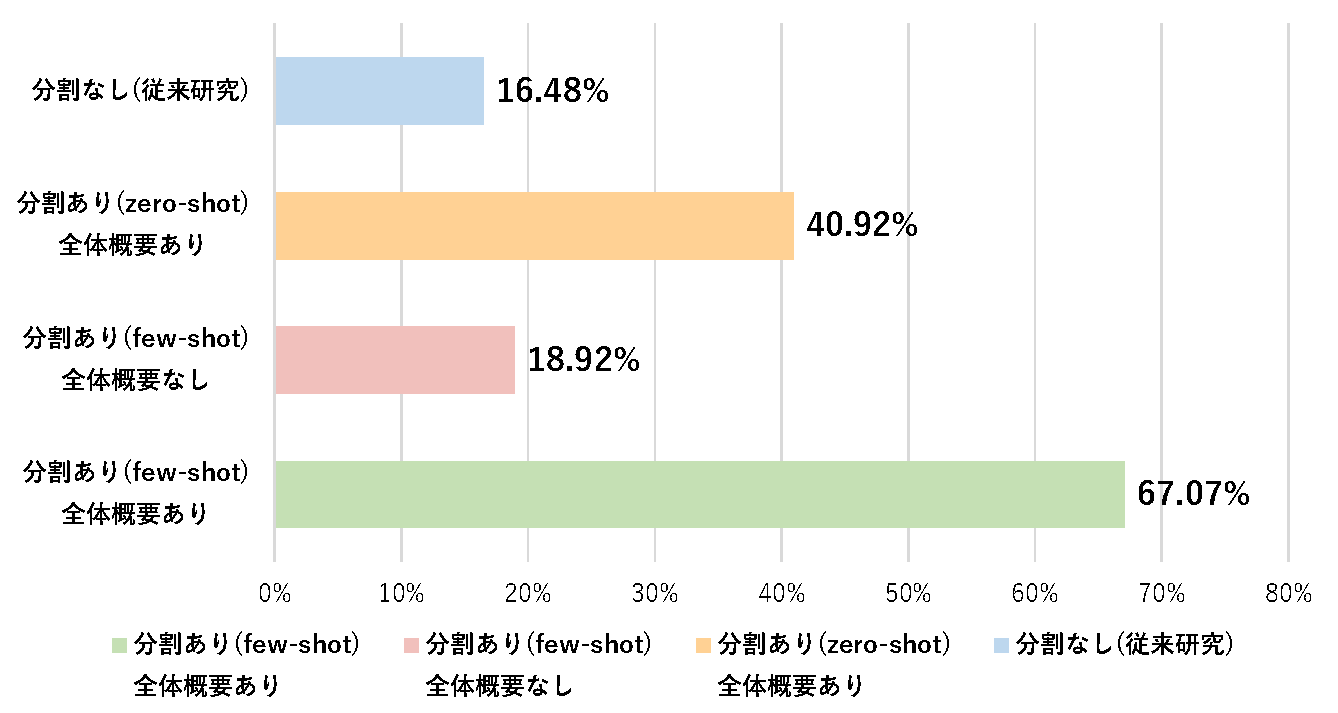
\includegraphics[width=1.0\linewidth]{./Toyoshima_fig/SIGSE_fig1.pdf}
    \caption{few-shotと全体概要の有無におけるテスト通過率比較}
    \label{ses2025}
\end{figure}

\subsection{RQ2}
統合前後でのテストは,合計で1,623件のテストが実施されたのに対して,要件の統合前の場合には67.84\%であるのに対して,統合後では68.76\%である事が確認された.又,統合前にテストを通過した/通過しなかったケースをそれぞれPassed/Failed,統合後にテストを通過した/通過しなかったケースをそれぞれPass/Failと定義した時の,それぞれの分布を図\ref{rq2_1}で示す.尚,本RQにおいてテストを通過する,とは問題単位で用意された入出力テストを全て通過したケースを指す.

PassedかつFailとなるケースは,要件の統合により「劣化」したケース,FailedかつPassとなるケースは,「改善」されたケースであり,それ以外の2項目は統合が生成されるコードの品質に影響を及ぼさなかったケースと考えられる.それぞれの割合を確認すると,劣化・改善がみられたのは全体の12.5\%であり,概ね変化がみられないことが確認された.

以上のことから,テスト通過率は概ね横ばいであり,通過する問題の構成も大きく変化しないことから,提案する統合手法は,生成されるコードの品質を損なわせるものではない事が示唆される.

\begin{figure}[t]
    \centering
    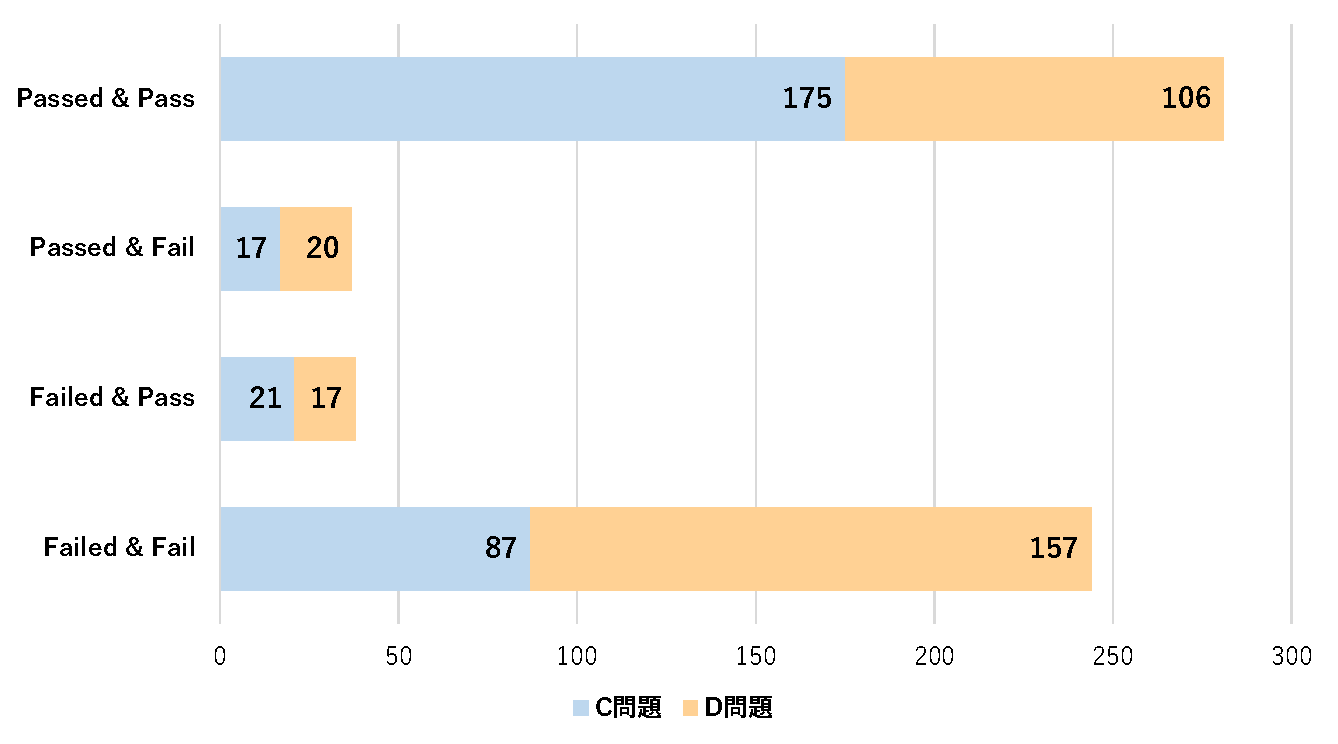
\includegraphics[width=1.0\linewidth]{./Toyoshima_fig/SIGSE_PF.pdf}
    \caption{few-shotと全体概要の有無におけるテスト通過率比較\protect\footnotemark}
    \label{rq2_1}
\end{figure}

\subsection{RQ3}
統合した結果,品質の劣化が発生しないことが確認されたことから,統合前後の両方でテストを通過したケース(Passed かつ Pass)のケースより8件の分割例と問題文を抽出し,few-shot学習と再分割を実施した.尚,分割例はC問題とD問題よりそれぞれ4問ずつ取得し,これらの問題は再分割・コード生成のデータセットからは除外し,それぞれ96問ずつで実験を実施した.RQ2で定義した問題単位のテスト結果の分布を図\ref{rq3_1}に示す.

用意されたテストを全て通過した問題数がC問題で252問,D問題で231問となり,総テスト通過率は83.85\%となることが確認された.又,改善が見られたケース(Failed かつ Pass)が全体の36\%と通過したテストの半分近くを占める結果となった.

以上より,本論文が提案する,統合に基づく要件の再分割は,要件に含まれる要求を正しく抽出できる可能性が示される.

\begin{figure}[t]
    \centering
    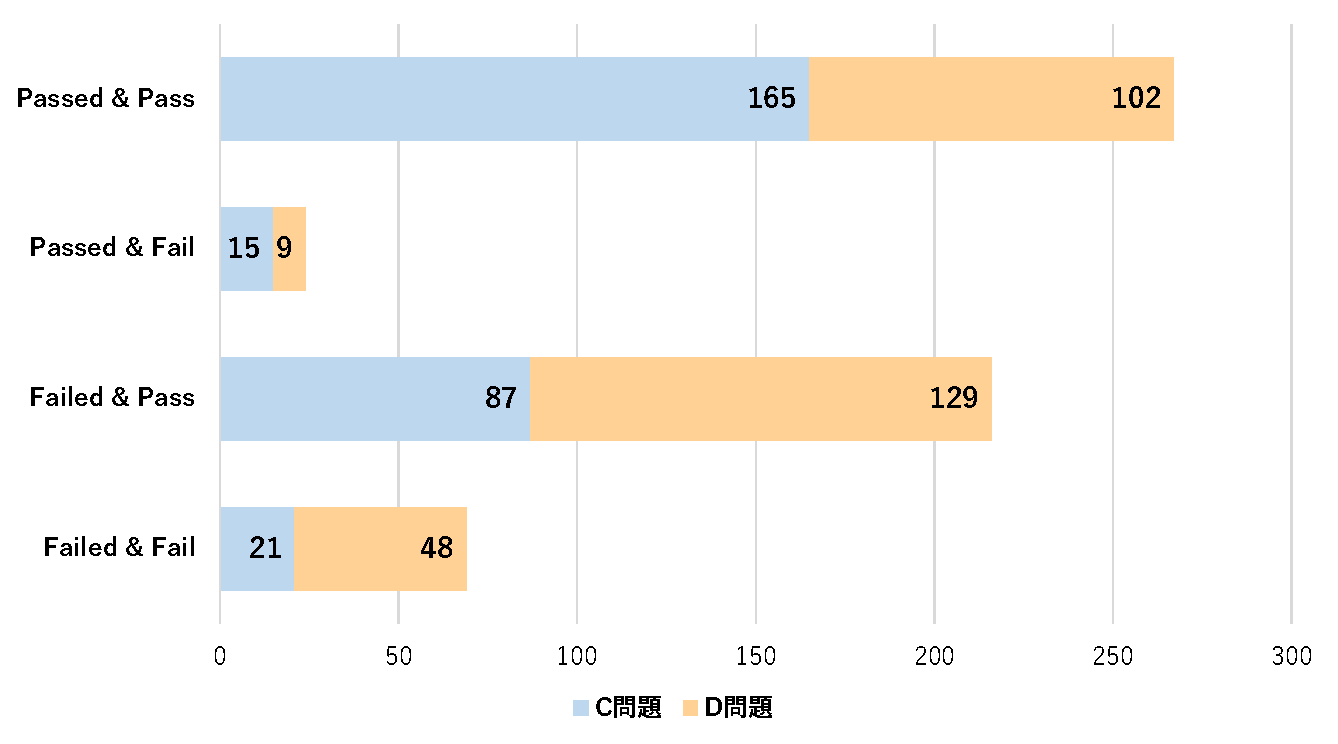
\includegraphics[width=1.0\linewidth]{./Toyoshima_fig/RQ3_1.pdf}
    \caption{few-shotと全体概要の有無におけるテスト通過率比較\protect\footnotemark}
    \label{rq3_1}
\end{figure}

%%%%%%%%%%%%%%%%%%%%%%%%%%%
%6
\section{考察}
\label{sec:discussion}
%%%%%%%%%%%%%%%%%%%%%%%%%%%
%6.1
\subsection{テスト通過率の向上した理由について考察\todo{サブタイ変更}}
ケーススタディ的に考えていく.


%6.1.1
\subsubsection{ケース1: 統合前・統合後・再分割後の全てでテストを通過したケース}
\memo{実際の分割例ってどこに置くか考える.付録か・・・?}
統合前の要件は,1つの要件あたりが変数の作成・初期化・値の格納や,関数の宣言などが要件の大部分を占めており,残りの大部分を少数の要件で定義する,という形式が確認された一方で,再分割後の要件では

%6.1.2
\subsubsection{ケース2: 再分割により改善が見られたケース}


%6.2
\subsection{妥当性の脅威}
田井くん背景は見られるが,モデル依存云々,LLM云々

%%%%%%%%%%%%%%%%%%%%%%%%%%%
%8
\section{おわりに}
\label{sec:conclusion}
%%%%%%%%%%%%%%%%%%%%%%%%%%%

\textbf{謝辞} ありがとうございました

\bibliographystyle{ipsjunsrt}
\bibliography{bibsample}

\end{document}

%memo
分割のやり直しでAI-likeな形式に変形された? イテレーション的に回していくコトでAフレンドリーな形式に変形される可能性について考察部分で持っていく